%\VignetteDepends{RcppOctave,rbenchmark}
%\VignetteCompiler{knitr}
%\VignetteEngine{knitr::knitr}

\documentclass[a4paper]{report}\usepackage[]{graphicx}\usepackage[]{color}
%% maxwidth is the original width if it is less than linewidth
%% otherwise use linewidth (to make sure the graphics do not exceed the margin)
\makeatletter
\def\maxwidth{ %
  \ifdim\Gin@nat@width>\linewidth
    \linewidth
  \else
    \Gin@nat@width
  \fi
}
\makeatother

\definecolor{fgcolor}{rgb}{0, 0, 0}
\newcommand{\hlnum}[1]{\textcolor[rgb]{0,0,0}{#1}}%
\newcommand{\hlstr}[1]{\textcolor[rgb]{0.741,0.553,0.545}{#1}}%
\newcommand{\hlcom}[1]{\textcolor[rgb]{0.675,0.125,0.125}{\textit{#1}}}%
\newcommand{\hlopt}[1]{\textcolor[rgb]{0,0,0}{#1}}%
\newcommand{\hlstd}[1]{\textcolor[rgb]{0,0,0}{#1}}%
\newcommand{\hlkwa}[1]{\textcolor[rgb]{0.612,0.125,0.933}{\textbf{#1}}}%
\newcommand{\hlkwb}[1]{\textcolor[rgb]{0.125,0.537,0.125}{#1}}%
\newcommand{\hlkwc}[1]{\textcolor[rgb]{0,0,1}{#1}}%
\newcommand{\hlkwd}[1]{\textcolor[rgb]{0,0,0}{#1}}%

\usepackage{framed}
\makeatletter
\newenvironment{kframe}{%
 \def\at@end@of@kframe{}%
 \ifinner\ifhmode%
  \def\at@end@of@kframe{\end{minipage}}%
  \begin{minipage}{\columnwidth}%
 \fi\fi%
 \def\FrameCommand##1{\hskip\@totalleftmargin \hskip-\fboxsep
 \colorbox{shadecolor}{##1}\hskip-\fboxsep
     % There is no \\@totalrightmargin, so:
     \hskip-\linewidth \hskip-\@totalleftmargin \hskip\columnwidth}%
 \MakeFramed {\advance\hsize-\width
   \@totalleftmargin\z@ \linewidth\hsize
   \@setminipage}}%
 {\par\unskip\endMakeFramed%
 \at@end@of@kframe}
\makeatother

\definecolor{shadecolor}{rgb}{.97, .97, .97}
\definecolor{messagecolor}{rgb}{0, 0, 0}
\definecolor{warningcolor}{rgb}{1, 0, 1}
\definecolor{errorcolor}{rgb}{1, 0, 0}
\newenvironment{knitrout}{}{} % an empty environment to be redefined in TeX

\let\hlesc\hlstd \let\hlpps\hlstd \let\hllin\hlstd \let\hlslc\hlcom
\usepackage{alltt}

% Style definition file generated by highlight 2.8, http://www.andre-simon.de/
% Highlighting theme definition:
%\newcommand{\hlopt}[1]{\textcolor[rgb]{0.1,0,0}{#1}}
%\newcommand{\hlstd}[1]{\textcolor[rgb]{0.17,0.48,0.2}{#1}}
%\newcommand{\hlnum}[1]{\textcolor[rgb]{0.88,0.1,0.44}{#1}}
%\newcommand{\hlesc}[1]{\textcolor[rgb]{0.79,0.29,0.89}{#1}}
%\newcommand{\hlstr}[1]{\textcolor[rgb]{0.79,0.29,0.89}{#1}}
%\newcommand{\hldstr}[1]{\textcolor[rgb]{0.79,0.29,0.89}{#1}}
%\newcommand{\hlslc}[1]{\textcolor[rgb]{0.12,0.64,0.07}{\it{#1}}}
%\newcommand{\hlcom}[1]{\textcolor[rgb]{0.12,0.64,0.07}{\it{#1}}}
%\newcommand{\hldir}[1]{\textcolor[rgb]{0.08,0.51,0.69}{#1}}
%\newcommand{\hlsym}[1]{\textcolor[rgb]{0.98,0.28,0}{#1}}
%\newcommand{\hlline}[1]{\textcolor[rgb]{0.47,0.09,0.72}{#1}}
%\newcommand{\hlkwa}[1]{\textcolor[rgb]{0.11,0.27,0.84}{\bf{#1}}}
%\newcommand{\hlkwb}[1]{\textcolor[rgb]{0.93,0.06,0.33}{\bf{#1}}}
%\newcommand{\hlkwc}[1]{\textcolor[rgb]{0.15,0.67,0.91}{\bf{#1}}}
%\newcommand{\hlkwd}[1]{\textcolor[rgb]{0.11,0.27,0.84}{#1}}
%\definecolor{bgcolor}{rgb}{1,0.98,0.73}



\usepackage{RJournal}
\usepackage[round]{natbib}
\bibliographystyle{abbrvnat}

%% load any required packages here
\usepackage{booktabs}
% define commands for notes
\usepackage{todonotes}
\newcommand{\devnote}[3]{\todo[inline, backgroundcolor=#1!20!white]{\scriptsize\textsf{\textbf{#2:} #3}}}
\newcommand{\dirk}[1]{\devnote{blue}{DE}{#1}}
\newcommand{\renaud}[1]{\devnote{red}{RG}{#1}}
\IfFileExists{upquote.sty}{\usepackage{upquote}}{}

\begin{document}

%% do not edit, for illustration only
\fancyhf{}
\fancyhead[LO,RE]{\textsc{Contributed Article}}
\fancyhead[RO,LE]{\thepage}
\fancyfoot[L]{The R Journal Vol. X/Y, Month, Year}
\fancyfoot[R]{ISSN 2073-4859}

%% replace RJtemplate with your article
\begin{article}

%% evaluate/include actual manuscript




\title{RcppOctave: Running Octave from R}
\author{by Dirk Eddelbuettel and Renaud Gaujoux}

\maketitle

\abstract{
  The \pkg{RcppOctave} package connects Octave to R, allowing R user to
  access another numerical computing language from within R.
  \dirk{TODO: Expand}
}

\section{Introduction}

Octave \citep{Octave:2012} is an interactive language that is primarily
intended for numerical computations. It is mostly compatible with Matlab
\citep{MATLAB:2010} and has found widespread adoption across different
disciplines. This include domains in which Matlab has historically been
pre-eminent such as applied mathematics, electrical engineering and signal
processing, but also in other fields such as machine learning,
bioinformatics, and finance.  Consequently, a large corpus of application
programs are available as \code{.m}-files (named after the commonly-chose
file extension) for which Octave provides an open source engine.

R \citep{R:2012}, a language and environment for statistical
computing and graphics, has become the dominant language for statistical
research, and a widely-used environment for empirical work in a variety of
fields.

While both languages share commonalities, their respective focus is different
making a combination of both environments an even more compelling choice.
This short paper illustrates the \pkg{RcppOctave} package by
\cite{CRAN:RcppOctave} which implements an interface between both these
environments.
\dirk{TODO: Better split between intro and next section}

\section{Octave}

Octave \citep{Octave:2012} is a powerful interactive language ``not unlike
Matlab'' and described in detail by \citet{Eaton:2008}. Octave can do
arithmetic for real, complex or integer-valued scalars and matrices, solve
sets of nonlinear algebraic equations, integrate functions over finite and
infinite intervals, and integrate systems of ordinary differential and
differential-algebraic equations.  Given the popularity of Matlab, Octave has
always had a lot of appeal in fields in which Matlab is popular.

As a simple illustration, consider the function below which converts two
arguments `distance' (in miles) and `time' (in minutes and seconds) into a
pace expressed as minutes-per-mile:

{ \small
%% by hand:  %% highlight --enclose-pre --no-doc --out-format=latex --syntax=Matlab --style=edit-emacs
\definecolor{shadecolor}{rgb}{1, 1, 1}\begin{kframe}\noindent
\ttfamily
\hlstd{}\hlslc{\#\#\ usage:}\hlstd{\ \ }\hlslc{p\ =\ pace\ (dist,\ time)}\hspace*{\fill}\\
\hlstd{}\hlkwa{function\ }\hlstd{p\ }\hlopt{=\ }\hlstd{}\hlkwd{pace\ }\hlstd{}\hlopt{(}\hlstd{dist}\hlopt{,\ }\hlstd{time}\hlopt{)}\hspace*{\fill}\\
\hlstd{}\hlstd{\ \ }\hlstd{}\hlkwd{if\ }\hlstd{}\hlopt{(}\hlstd{nargin\ }\hlopt{$<$\ }\hlstd{}\hlnum{2}\hlstd{}\hlopt{)}\hspace*{\fill}\\
\hlstd{}\hlstd{\ \ \ \ }\hlstd{}\hlkwd{usage}\hlstd{}\hlopt{(}\hlstd{}\hlstr{"Call\ as\ pace\ (dist,\ time)"}\hlstd{}\hlopt{)}\hspace*{\fill}\\
\hlstd{}\hlstd{\ \ }\hlstd{}\hlkwa{end}\hspace*{\fill}\\
\hlstd{\hspace*{\fill}\\
}\hlstd{\ \ }\hlstd{}\hlslc{\#\#\ total\ seconds}\hspace*{\fill}\\
\hlstd{}\hlstd{\ \ }\hlstd{a\ }\hlopt{=\ }\hlstd{}\hlkwc{floor}\hlstd{}\hlopt{(}\hlstd{time}\hlopt{){*}}\hlstd{}\hlnum{60\ }\hlstd{}\hlopt{+\ (}\hlstd{time}\hlopt{{-}}\hlstd{}\hlkwc{floor}\hlstd{}\hlopt{(}\hlstd{time}\hlopt{)){*}}\hlstd{}\hlnum{100}\hlstd{}\hlopt{;}\hspace*{\fill}\\
\hlstd{}\hlstd{\ \ }\hlstd{}\hlslc{\#\#\ seconds\ per\ miles}\hspace*{\fill}\\
\hlstd{}\hlstd{\ \ }\hlstd{b\ }\hlopt{=\ }\hlstd{a\ }\hlopt{/\ }\hlstd{dist}\hlopt{;}\hspace*{\fill}\\
\hlstd{}\hlstd{\ \ }\hlstd{}\hlslc{\#\#\ minutes\ per\ mile}\hspace*{\fill}\\
\hlstd{}\hlstd{\ \ }\hlstd{c\ }\hlopt{=\ }\hlstd{}\hlkwc{floor}\hlstd{}\hlopt{(}\hlstd{b}\hlopt{/}\hlstd{}\hlnum{60}\hlstd{}\hlopt{);}\hspace*{\fill}\\
\hlstd{}\hlstd{\ \ }\hlstd{}\hlslc{\#\#\ seconds\ per\ mile}\hspace*{\fill}\\
\hlstd{}\hlstd{\ \ }\hlstd{d\ }\hlopt{=\ }\hlstd{b\ }\hlopt{{-}\ }\hlstd{c}\hlopt{{*}}\hlstd{}\hlnum{60}\hlstd{}\hlopt{;}\hspace*{\fill}\\
\hlstd{\hspace*{\fill}\\
}\hlstd{\ \ }\hlstd{p\ }\hlopt{=\ }\hlstd{c\ }\hlopt{+\ }\hlstd{d}\hlopt{/}\hlstd{}\hlnum{100}\hlstd{}\hlopt{;}\hspace*{\fill}\\
\hlstd{}\hlstd{\ \ }\hlstd{}\hlkwd{printf}\hlstd{}\hlopt{(}\hlstd{}\hlstr{"\%.2f\ over\ \%.2f\ is\ \%d:\%d\ aka\ \%.2f}\hlesc{$\backslash$n}\hlstr{"}\hlstd{}\hlopt{,}\hspace*{\fill}\\
\hlstd{}\hlstd{\ \ \ \ \ \ \ \ \ }\hlstd{time}\hlopt{,\ }\hlstd{dist}\hlopt{,\ }\hlstd{c}\hlopt{,\ }\hlstd{d}\hlopt{,\ }\hlstd{p}\hlopt{);}\hspace*{\fill}\\
\hlstd{}\hlkwa{endfunction}\hlstd{}\hspace*{\fill}
\mbox{}
\normalfont
\normalsize
\end{kframe}

}

The example shows a few subtle difference between Octave and Matlab. Comments
starts with hash sign. Default function help is provided before the function
definition. The \code{endfunction} keyword ends a function.

It also shows how the semicolon at the end of lines is used to suppress
output; expression not ending in a semi-colon print their final result.

%\section{Example: Matrix Operations}  % or something else

%TODO: Show two or three simple call illustrating the variable arguments etc.

Octave is particularly useful for linear algebra and calculations involving
matrices and vectors.  For multiplication, the \code{*} symbol is
overloaded. For example, for a row-vector $a$, the expressions \code{a * a'}
amd \code{a' * a} compute, respectively the (scalar) inner product and matrix
outer product as the apostrophe invokes a tranposition. Common matrix
functions such as \code{eig} or \code{det} are available as well.  For more
complete example in provided in the next section.

\renaud{TODO: A few words about RcppOctave, Design, Limitations, ...}

\section{Example: Kalman Filter}

\cite{Eddelbuettel+Sanderson:2013} introduce the \pkg{RcppArmadillo} package
and illustrate it via an example comparing a Kalman filter implementation in both R and
C++. As the code underlying this example was initially published for
Matlab\footnote{See
  \url{http://www.mathworks.com/products/matlab-coder/demos.html?file=/products/demos/shipping/coder/coderdemo_kalman_filter.html}.},
it can of course also be used with RcppOctave.

\dirk{TODO: Few words about the example}

{ \small
%% by hand:  %% highlight --enclose-pre --no-doc --out-format=latex --syntax=Matlab --style=edit-emacs
\definecolor{shadecolor}{rgb}{1, 1, 1}\begin{kframe}\noindent
\ttfamily
\hlstd{}\hlkwa{function\ }\hlstd{Y\ }\hlopt{=\ }\hlstd{kalmanM}\hlopt{(}\hlstd{pos}\hlopt{)}\hspace*{\fill}\\
\hlstd{}\hlstd{\ \ }\hlstd{dt}\hlopt{=}\hlstd{}\hlnum{1}\hlstd{}\hlopt{;}\hspace*{\fill}\\
\hlstd{}\hlstd{\ \ }\hlstd{}\hlslc{\%\%\ Initialize\ state\ transition\ matrix}\hspace*{\fill}\\
\hlstd{}\hlstd{\ \ }\hlstd{A}\hlopt{={[}\ }\hlstd{}\hlnum{1\ 0\ }\hlstd{dt\ }\hlnum{0\ 0\ 0}\hlstd{}\hlopt{;}\hlstd{...}\hlstd{\ \ \ \ \ }\hlstd{}\hlslc{\%\ {[}x}\hlstd{\ \ }\hlslc{{]}}\hspace*{\fill}\\
\hlstd{}\hlstd{\ \ \ \ \ \ }\hlstd{}\hlnum{0\ 1\ 0\ }\hlstd{dt\ }\hlnum{0\ 0}\hlstd{}\hlopt{;}\hlstd{...}\hlstd{\ \ \ \ \ }\hlstd{}\hlslc{\%\ {[}y}\hlstd{\ \ }\hlslc{{]}}\hspace*{\fill}\\
\hlstd{}\hlstd{\ \ \ \ \ \ }\hlstd{}\hlnum{0\ 0\ 1\ 0\ }\hlstd{dt\ }\hlnum{0}\hlstd{}\hlopt{;}\hlstd{...}\hlstd{\ \ \ \ \ }\hlstd{}\hlslc{\%\ {[}Vx{]}}\hspace*{\fill}\\
\hlstd{}\hlstd{\ \ \ \ \ \ }\hlstd{}\hlnum{0\ 0\ 0\ 1\ 0\ }\hlstd{dt}\hlopt{;}\hlstd{...}\hlstd{\ \ \ \ \ }\hlstd{}\hlslc{\%\ {[}Vy{]}}\hspace*{\fill}\\
\hlstd{}\hlstd{\ \ \ \ \ \ }\hlstd{}\hlnum{0\ 0\ 0\ 0\ 1\ 0\ }\hlstd{}\hlopt{;}\hlstd{...}\hlstd{\ \ \ \ \ }\hlstd{}\hlslc{\%\ {[}Ax{]}}\hspace*{\fill}\\
\hlstd{}\hlstd{\ \ \ \ \ \ }\hlstd{}\hlnum{0\ 0\ 0\ 0\ 0\ 1\ }\hlstd{}\hlopt{{]};}\hlstd{\ \ \ \ \ \ \ }\hlopt{}\hlstd{}\hlslc{\%\ {[}Ay{]}}\hspace*{\fill}\\
\hlstd{\hspace*{\fill}\\
}\hlstd{\ \ }\hlstd{}\hlslc{\%\ Initialize\ measurement\ matrix}\hspace*{\fill}\\
\hlstd{}\hlstd{\ \ }\hlstd{H\ }\hlopt{=\ {[}\ }\hlstd{}\hlnum{1\ 0\ 0\ 0\ 0\ 0}\hlstd{}\hlopt{;\ }\hlstd{}\hlnum{0\ 1\ 0\ 0\ 0\ 0\ }\hlstd{}\hlopt{{]};}\hspace*{\fill}\\
\hlstd{\hspace*{\fill}\\
}\hlstd{\ \ }\hlstd{Q\ }\hlopt{=\ }\hlstd{eye}\hlopt{(}\hlstd{}\hlnum{6}\hlstd{}\hlopt{);}\hspace*{\fill}\\
\hlstd{}\hlstd{\ \ }\hlstd{R\ }\hlopt{=\ }\hlstd{}\hlnum{1000\ }\hlstd{}\hlopt{{*}\ }\hlstd{eye}\hlopt{(}\hlstd{}\hlnum{2}\hlstd{}\hlopt{);}\hspace*{\fill}\\
\hlstd{\hspace*{\fill}\\
}\hlstd{\ \ }\hlstd{x\textunderscore est\ }\hlopt{=\ }\hlstd{zeros}\hlopt{(}\hlstd{}\hlnum{6}\hlstd{}\hlopt{,\ }\hlstd{}\hlnum{1}\hlstd{}\hlopt{);}\hspace*{\fill}\\
\hlstd{}\hlstd{\ \ }\hlstd{p\textunderscore est\ }\hlopt{=\ }\hlstd{zeros}\hlopt{(}\hlstd{}\hlnum{6}\hlstd{}\hlopt{,\ }\hlstd{}\hlnum{6}\hlstd{}\hlopt{);}\hspace*{\fill}\\
\hlstd{\hspace*{\fill}\\
}\hlstd{\ \ }\hlstd{numPts\ }\hlopt{=\ }\hlstd{}\hlkwa{size}\hlstd{}\hlopt{(}\hlstd{pos}\hlopt{,}\hlstd{}\hlnum{1}\hlstd{}\hlopt{);}\hspace*{\fill}\\
\hlstd{}\hlstd{\ \ }\hlstd{Y\ }\hlopt{=\ }\hlstd{zeros}\hlopt{(}\hlstd{numPts}\hlopt{,\ }\hlstd{}\hlnum{2}\hlstd{}\hlopt{);}\hspace*{\fill}\\
\hlstd{\hspace*{\fill}\\
}\hlstd{\ \ }\hlstd{}\hlkwa{for\ }\hlstd{idx\ }\hlopt{=\ }\hlstd{}\hlnum{1}\hlstd{}\hlopt{:}\hlstd{numPts\hspace*{\fill}\\
}\hlstd{\ \ \ \ }\hlstd{z\ }\hlopt{=\ }\hlstd{pos}\hlopt{(}\hlstd{idx}\hlopt{,\ :)}\hlstd{'}\hlopt{;}\hspace*{\fill}\\
\hlstd{\hspace*{\fill}\\
}\hlstd{\ \ \ \ }\hlstd{}\hlslc{\%\%\ Predicted\ state\ and\ covariance}\hspace*{\fill}\\
\hlstd{}\hlstd{\ \ \ \ }\hlstd{x\textunderscore prd\ }\hlopt{=\ }\hlstd{A\ }\hlopt{{*}\ }\hlstd{x\textunderscore est}\hlopt{;}\hspace*{\fill}\\
\hlstd{}\hlstd{\ \ \ \ }\hlstd{p\textunderscore prd\ }\hlopt{=\ }\hlstd{A\ }\hlopt{{*}\ }\hlstd{p\textunderscore est\ }\hlopt{{*}\ }\hlstd{A'\ }\hlopt{+\ }\hlstd{Q}\hlopt{;}\hspace*{\fill}\\
\hlstd{}\hlstd{\ \ \ \ }\hlstd{}\hlslc{\%\%\ Estimation}\hspace*{\fill}\\
\hlstd{}\hlstd{\ \ \ \ }\hlstd{S\ }\hlopt{=\ }\hlstd{H\ }\hlopt{{*}\ }\hlstd{p\textunderscore prd'\ }\hlopt{{*}\ }\hlstd{H'\ }\hlopt{+\ }\hlstd{R}\hlopt{;}\hspace*{\fill}\\
\hlstd{}\hlstd{\ \ \ \ }\hlstd{B\ }\hlopt{=\ }\hlstd{H\ }\hlopt{{*}\ }\hlstd{p\textunderscore prd'}\hlopt{;}\hspace*{\fill}\\
\hlstd{}\hlstd{\ \ \ \ }\hlstd{klm\textunderscore gain\ }\hlopt{=\ (}\hlstd{S\ $\backslash$\ B}\hlopt{)}\hlstd{'}\hlopt{;}\hspace*{\fill}\\
\hlstd{}\hlstd{\ \ \ \ }\hlstd{}\hlslc{\%\%\ Estimated\ state\ and\ covariance}\hspace*{\fill}\\
\hlstd{}\hlstd{\ \ \ \ }\hlstd{x\textunderscore est\ }\hlopt{=\ }\hlstd{x\textunderscore prd\ }\hlopt{+\ }\hlstd{klm\textunderscore gain\ }\hlopt{{*}\ (}\hlstd{z\ }\hlopt{{-}\ }\hlstd{H\ }\hlopt{{*}\ }\hlstd{x\textunderscore prd}\hlopt{);}\hspace*{\fill}\\
\hlstd{}\hlstd{\ \ \ \ }\hlstd{p\textunderscore est\ }\hlopt{=\ }\hlstd{p\textunderscore prd\ }\hlopt{{-}\ }\hlstd{klm\textunderscore gain\ }\hlopt{{*}\ }\hlstd{H\ }\hlopt{{*}\ }\hlstd{p\textunderscore prd}\hlopt{;}\hspace*{\fill}\\
\hlstd{}\hlstd{\ \ \ \ }\hlstd{}\hlslc{\%\%\ Compute\ the\ estimated\ measurements}\hspace*{\fill}\\
\hlstd{}\hlstd{\ \ \ \ }\hlstd{Y}\hlopt{(}\hlstd{idx}\hlopt{,\ :)\ =\ }\hlstd{H\ }\hlopt{{*}\ }\hlstd{x\textunderscore est}\hlopt{;}\hspace*{\fill}\\
\hlstd{}\hlstd{\ \ }\hlstd{}\hlkwa{end}\hlstd{\ \ \ \ \ \ \ \ \ \ \ \ \ \ \ \ }\hlkwa{}\hlstd{}\hlslc{\%\ of\ the\ function}\hspace*{\fill}\\
\hlstd{}\hlkwa{end}\hlstd{\ \ \ }\hlkwa{}\hlstd{}\hlslc{\%\ of\ the\ function}\hlstd{}\hspace*{\fill}
\mbox{}
\normalfont
\normalsize
\end{kframe}

}

This function, along with several R implementations, is provided in the
\pkg{RcppOctave} package as \code{demo(Kalman)}.
Table~\ref{tab:benchmark} summaries the performance.

%                 test replications elapsed relative
% 7  KalmanOctave(pos)          100   3.943  1.00000
% 2      KalmanRC(pos)          100   5.987  1.51839
% 1       KalmanR(pos)          100   6.047  1.53360
% 4   KalmanRfunC(pos)          100   6.262  1.58813
% 3    KalmanRfun(pos)          100   6.648  1.68603
% 6 FirstKalmanRC(pos)          100   8.992  2.28050
% 5  FirstKalmanR(pos)          100   9.405  2.38524

\begin{table}[tb]
  \begin{center}
    \begin{small}
      \begin{tabular}{lrr}
        \toprule
        {\bf Implementation \phantom{XX}} & {\bf Time in sec.} & {\bf Rel.~ to best} \\
        \cmidrule(r){1-3}
        %% original times, Summer 2012
        %%  KalmanOctave  & 3.943 & 1.000 \\
        %%      KalmanRC  & 5.987 & 1.518 \\
        %%       KalmanR  & 6.047 & 1.534 \\
        %%   KalmanRfunC  & 6.262 & 1.588 \\
        %%    KalmanRfun  & 6.648 & 1.686 \\
        %% FirstKalmanRC  & 8.992 & 2.281 \\
        %%  FirstKalmanR  & 9.405 & 2.385 \\
         KalmanOctave  & 1.93 & 1.00 \\
          KalmanRfunC  & 4.99 & 2.59 \\
             KalmanRC  & 5.13 & 2.66 \\
           KalmanRfun  & 5.45 & 2.83 \\
              KalmanR  & 5.46 & 2.83 \\
        FirstKalmanRC  & 6.41 & 3.32 \\
         FirstKalmanR  & 6.84 & 3.54 \\
         \bottomrule
      \end{tabular}
      \caption{Performance comparison of various implementations of a Kalman filter.
        KalmanOctave is the \pkg{RcppOctave} based implementation shown above.
        KalmanR is the \R implementation using an environment; KalmanRfun use a
        function; FirstKalmanR is a direct translation of the original Matlab
        implementation; versions ending in C are the byte-compiled variants of
        the respective version.  Timings are averaged over 100 replications.
        The comparison was made using R version 2.15.2, Rcpp version 0.10.2 and
        RcppOctave version 0.8.14 on Ubuntu 12.10 running in 64-bit mode on a
        2.67 GHz Intel i7 processor.}
      \label{tab:benchmark}
    \end{small}
  \end{center}
\end{table}

\dirk{TODO: More about the example, performance comparison, knocking socks off R}


\section{Example: Reproducible Random Numbers}

\dirk{TODO: Reference from his repeated blog posts}
Wilkinson used a simple bivariate Gibbs Sampler as a basis for comparisons
between different programming languages such as C, Java, Python and R. His
example has been re-used in number of other presentations.

We can adapt this example here as it provides a suitable framework for
showing how \pkg{RcppOctave} can interact with the random number generators
in R.

%DE: Super-useful feature, but shall we have that here or as part of the Gibbs sampler comparison
\dirk{TODO: Make true Gibbs sampler example}
{\small
\begin{knitrout}
\definecolor{shadecolor}{rgb}{1, 1, 1}\color{fgcolor}\begin{kframe}
\begin{alltt}
\hlkwd{library}\hlstd{(RcppOctave)}
\hlkwd{set.seed}\hlstd{(}\hlnum{1}\hlstd{)}     \hlcom{# reset the R RNG}
\hlstd{a} \hlkwb{<-} \hlkwd{runif}\hlstd{(}\hlnum{10}\hlstd{)}
\hlcom{# define octave function}
\hlkwd{o_source}\hlstd{(}\hlkwc{text}\hlstd{=}\hlstr{"
   function [x] = orng(n)
      x = rand(1, n);
   end
"}\hlstd{)}
\hlkwd{set.seed}\hlstd{(}\hlnum{1}\hlstd{)}     \hlcom{# reset the R RNG}
\hlkwd{identical}\hlstd{(.O}\hlopt{$}\hlkwd{orng}\hlstd{(}\hlnum{10}\hlstd{), a)}
\end{alltt}
\begin{verbatim}
## [1] TRUE
\end{verbatim}
\end{kframe}
\end{knitrout}

}

In this example, we first draw ten random number distributed $U(0,1)$ using
the default generator in R. We then define an Octave function from R. Similar
to how the \pkg{inline} package \citep{CRAN:inline} handles C or C++ code, we
simply define a character string which then passed the Octave interpreter via
the \verb|o_source()| function.  We re-set the seed of the underlying RNG in
R and call our Octave function. As it actually calls back into the RNG from
R, our two vectors are the same.  This is a critically important feature to
ensure reproducibility.

We can also define functions which draws from the Gamma distribution:
{\small
%## we have  'randg(a, N)/b' == rgamma(a,b)
%## CORRECTION:  set.seed(42); .O$gam(2,3)
%##         ==   set.seed(42); rgamma(1,2,1,3)
%##         ==   set.seed(42); rgamma(1,2,1)*3
\begin{knitrout}
\definecolor{shadecolor}{rgb}{1, 1, 1}\color{fgcolor}\begin{kframe}
\begin{alltt}
\hlcom{## define a Gamma RNG draw function}
\hlkwd{o_source}\hlstd{(}\hlkwc{text}\hlstd{=}\hlstr{"
  ## gamma(a,b) of dim. n by 1
  function x = orngg(a, b, n)
    x = b * randg(a, n, 1);
  end
"}\hlstd{)}
\hlkwd{set.seed}\hlstd{(}\hlnum{42}\hlstd{)}
\hlstd{N} \hlkwb{<-} \hlnum{50000}
\hlstd{x1} \hlkwb{<-} \hlkwd{c}\hlstd{(.O}\hlopt{$}\hlkwd{orngg}\hlstd{(}\hlnum{9}\hlstd{,}\hlnum{1}\hlstd{,N))}
\hlstd{x2} \hlkwb{<-} \hlkwd{c}\hlstd{(.O}\hlopt{$}\hlkwd{orngg}\hlstd{(}\hlnum{4}\hlstd{,}\hlnum{1}\hlstd{,N))}
\hlstd{x3} \hlkwb{<-} \hlkwd{c}\hlstd{(.O}\hlopt{$}\hlkwd{orngg}\hlstd{(}\hlnum{1}\hlstd{,}\hlnum{4}\hlstd{,N))}
\hlkwd{plot}\hlstd{(}\hlkwd{density}\hlstd{(x1),} \hlkwc{main}\hlstd{=}\hlstr{"Calling from Octave"}\hlstd{,}
     \hlkwc{col}\hlstd{=}\hlstr{"orange"}\hlstd{,} \hlkwc{ylim}\hlstd{=}\hlkwd{c}\hlstd{(}\hlnum{0}\hlstd{,}\hlnum{0.23}\hlstd{),} \hlkwc{xlim}\hlstd{=}\hlkwd{c}\hlstd{(}\hlopt{-}\hlnum{1}\hlstd{,}\hlnum{22}\hlstd{))}
\hlkwd{lines}\hlstd{(}\hlkwd{density}\hlstd{(x2),} \hlkwc{col}\hlstd{=}\hlstr{'mediumblue'}\hlstd{)}
\hlkwd{lines}\hlstd{(}\hlkwd{density}\hlstd{(x3),} \hlkwc{col}\hlstd{=}\hlstr{'brown'}\hlstd{)}
\end{alltt}
\end{kframe}
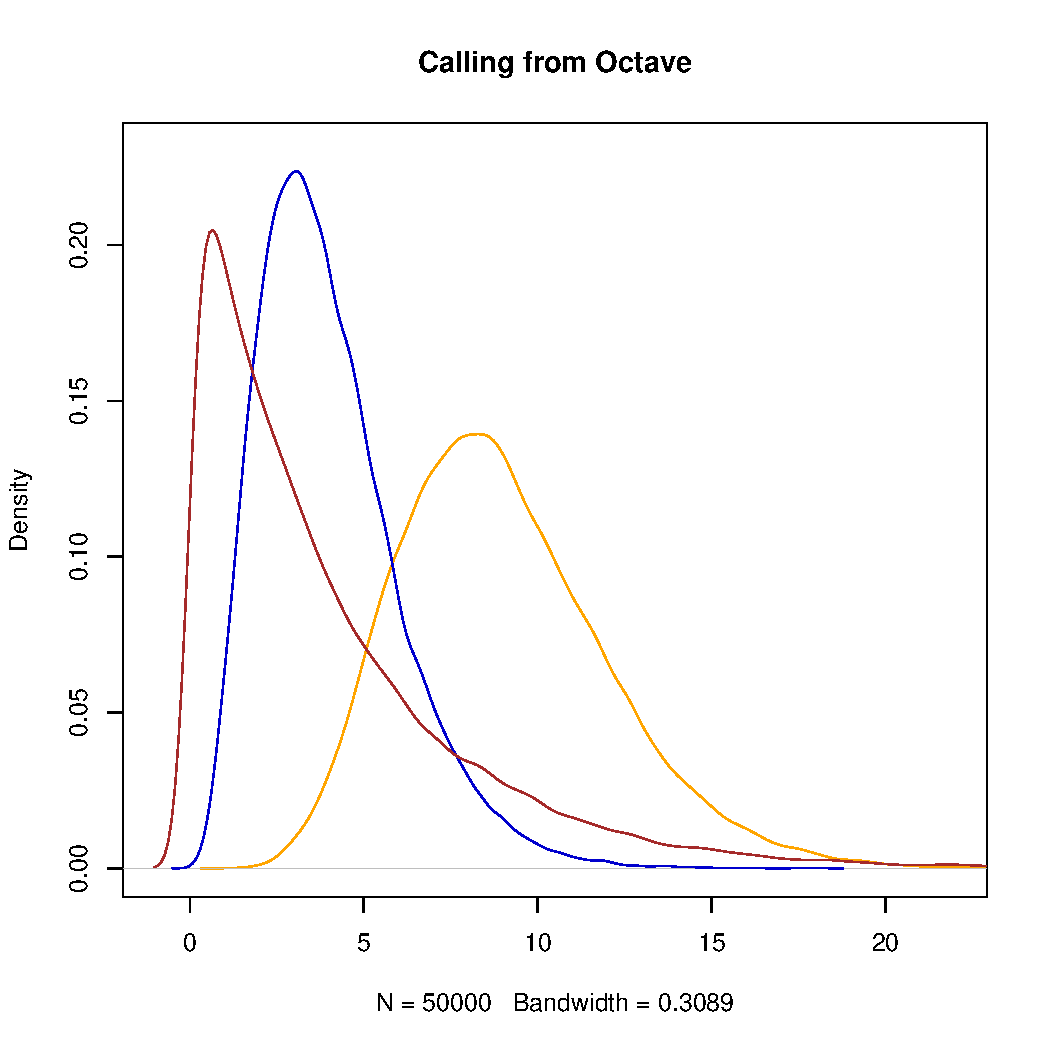
\includegraphics[width=\maxwidth]{/home/renaud/Documents/projects/RcppOctave/pkg/vignettes/figure/RJwrapper-rngGamma} 

\end{knitrout}

}

As \pkg{RcppOctave} ensures that Octave calls back into the R random-number
generator, we can generate the same chart directly from R:

{\small
\begin{knitrout}
\definecolor{shadecolor}{rgb}{1, 1, 1}\color{fgcolor}\begin{kframe}
\begin{alltt}
\hlkwd{set.seed}\hlstd{(}\hlnum{42}\hlstd{)}  \hlcom{# reset RNG}
\hlstd{N} \hlkwb{<-} \hlnum{50000}
\hlkwd{plot}\hlstd{(}\hlkwd{density}\hlstd{(}\hlkwd{rgamma}\hlstd{(N,}\hlnum{9}\hlstd{,}\hlnum{1}\hlstd{)),} \hlkwc{main}\hlstd{=}\hlstr{"Calling rgamma from R"}\hlstd{,}
     \hlkwc{col}\hlstd{=}\hlstr{"orange"}\hlstd{,} \hlkwc{ylim}\hlstd{=}\hlkwd{c}\hlstd{(}\hlnum{0}\hlstd{,}\hlnum{0.23}\hlstd{),} \hlkwc{xlim}\hlstd{=}\hlkwd{c}\hlstd{(}\hlopt{-}\hlnum{1}\hlstd{,}\hlnum{22}\hlstd{))}
\hlkwd{lines}\hlstd{(}\hlkwd{density}\hlstd{(}\hlkwd{rgamma}\hlstd{(N,}\hlnum{4}\hlstd{,}\hlnum{1}\hlstd{)),} \hlkwc{col}\hlstd{=}\hlstr{'mediumblue'}\hlstd{)}
\end{alltt}
\end{kframe}
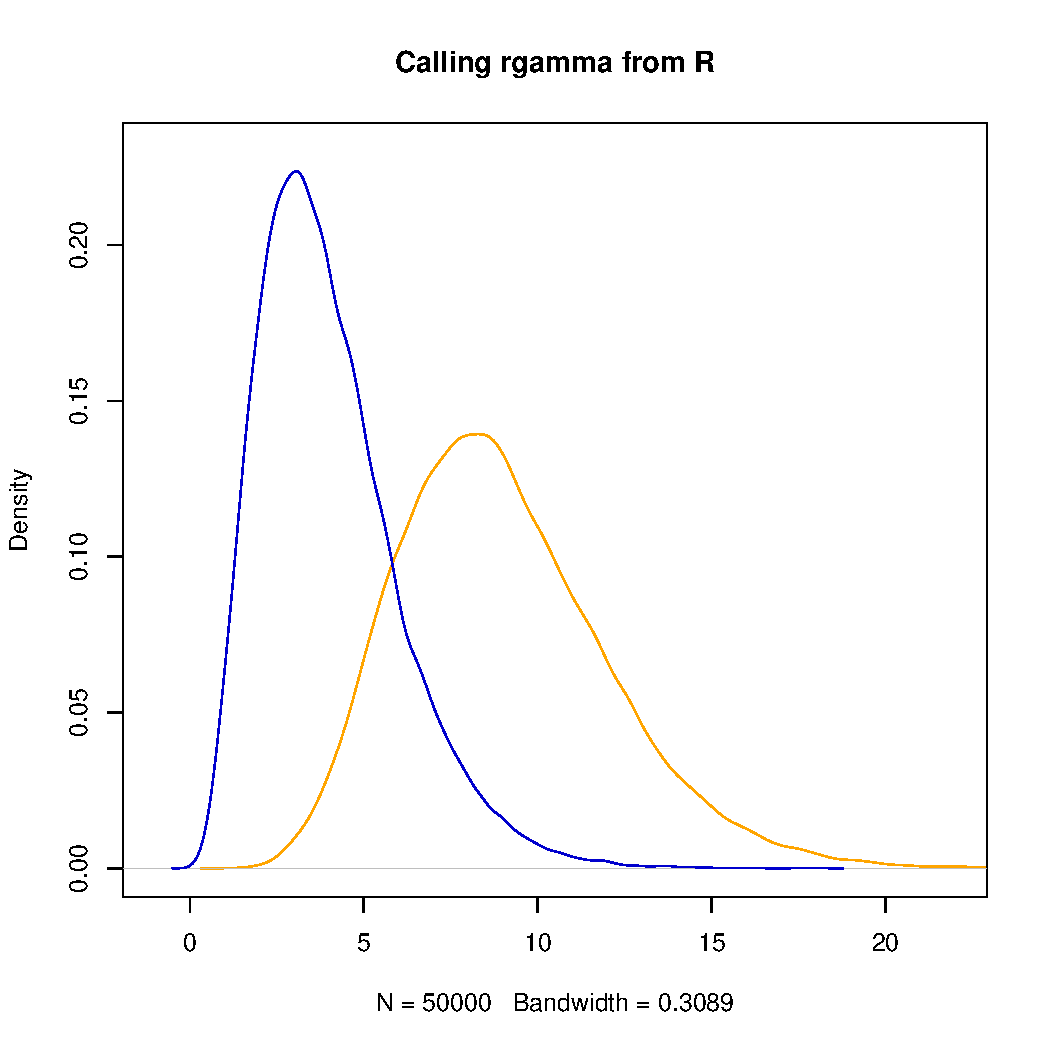
\includegraphics[width=\maxwidth]{/home/renaud/Documents/projects/RcppOctave/pkg/vignettes/figure/RJwrapper-rngGammaR} 
\begin{kframe}\begin{alltt}
\hlkwd{lines}\hlstd{(}\hlkwd{density}\hlstd{(}\hlkwd{rgamma}\hlstd{(N,}\hlnum{1}\hlstd{,}\hlnum{1}\hlstd{,}\hlnum{4}\hlstd{)),} \hlkwc{col}\hlstd{=}\hlstr{'brown'}\hlstd{)}
\end{alltt}


{\ttfamily\noindent\bfseries\color{errorcolor}{\#\# Error: specify 'rate' or 'scale' but not both}}\end{kframe}
\end{knitrout}

}

\bibliography{../inst/REFERENCES}

\address{Dirk Eddelbuettel \\
  Debian Project \\
  River Forest, IL\\
  USA}\\
\email{edd@debian.org}

\address{Renaud Gaujoux \\
  Computational Biology \\
  University of Cape Town \\
  Cape Town \\
  South Africa}\\
\email{renaud@cbio.uct.ac.za}

%%% Local Variables:
%%% mode: latex
%%% TeX-master: "RJwrapper"
%%% End:

\end{article}

\end{document}
